% 
% WebCrypto
% @author Pieter Maene <pieter.maene@student.kuleuven.be>
%

\chapter{Web Cryptography API}
\label{chap:web_cryptography_api}

Wanneer webontwikkelaars vandaag cryptografische functies nodig hebben in hun toepassingen, moeten ze bijna JavaScript gebruiken omwille van compatibiliteit. Hoewel er de laatste jaren zeer grote vooruitgang geboekt is, zullen de meeste JavaScript engines nog steeds minder goed presteren dan native code.\cite{site:resig_javascript_performance_rundown}\cite{site:cois_javascript_performance_rundown_2012}\cite{smedberg_performance_analysis_of_javascript} De W3C startte in 2012 een working group op om een nieuwe browser API te defini\"eren: de Web Cryptography API.\cite{wiki:webcrypto}

\npar In \ref{sec:wc:wb_cryptography_api} wordt deze nieuwe API kort besproken. Daarna wordt in \ref{sec:wc:nfwebcrypto} gekeken naar de NfWebCrypto polyfill, die de nieuwe functionaliteit implementeert in een plugin voor Google Chrome. Tot slot wordt deze implementatie in \ref{sec:wc:benchmarks} vergeleken met bestaande cryptografische libraries.

\section{Web Cryptography API~\cite{sleevi_watson_web_cryptography_api}}
\label{sec:wc:wb_cryptography_api}

\section{NfWebCrypto}
\label{sec:wc:nfwebcrypto}

\section{Benchmarks}
\label{sec:wc:benchmarks}

\subsection{Modulaire exponentiatie}

\begin{figure}
  \center{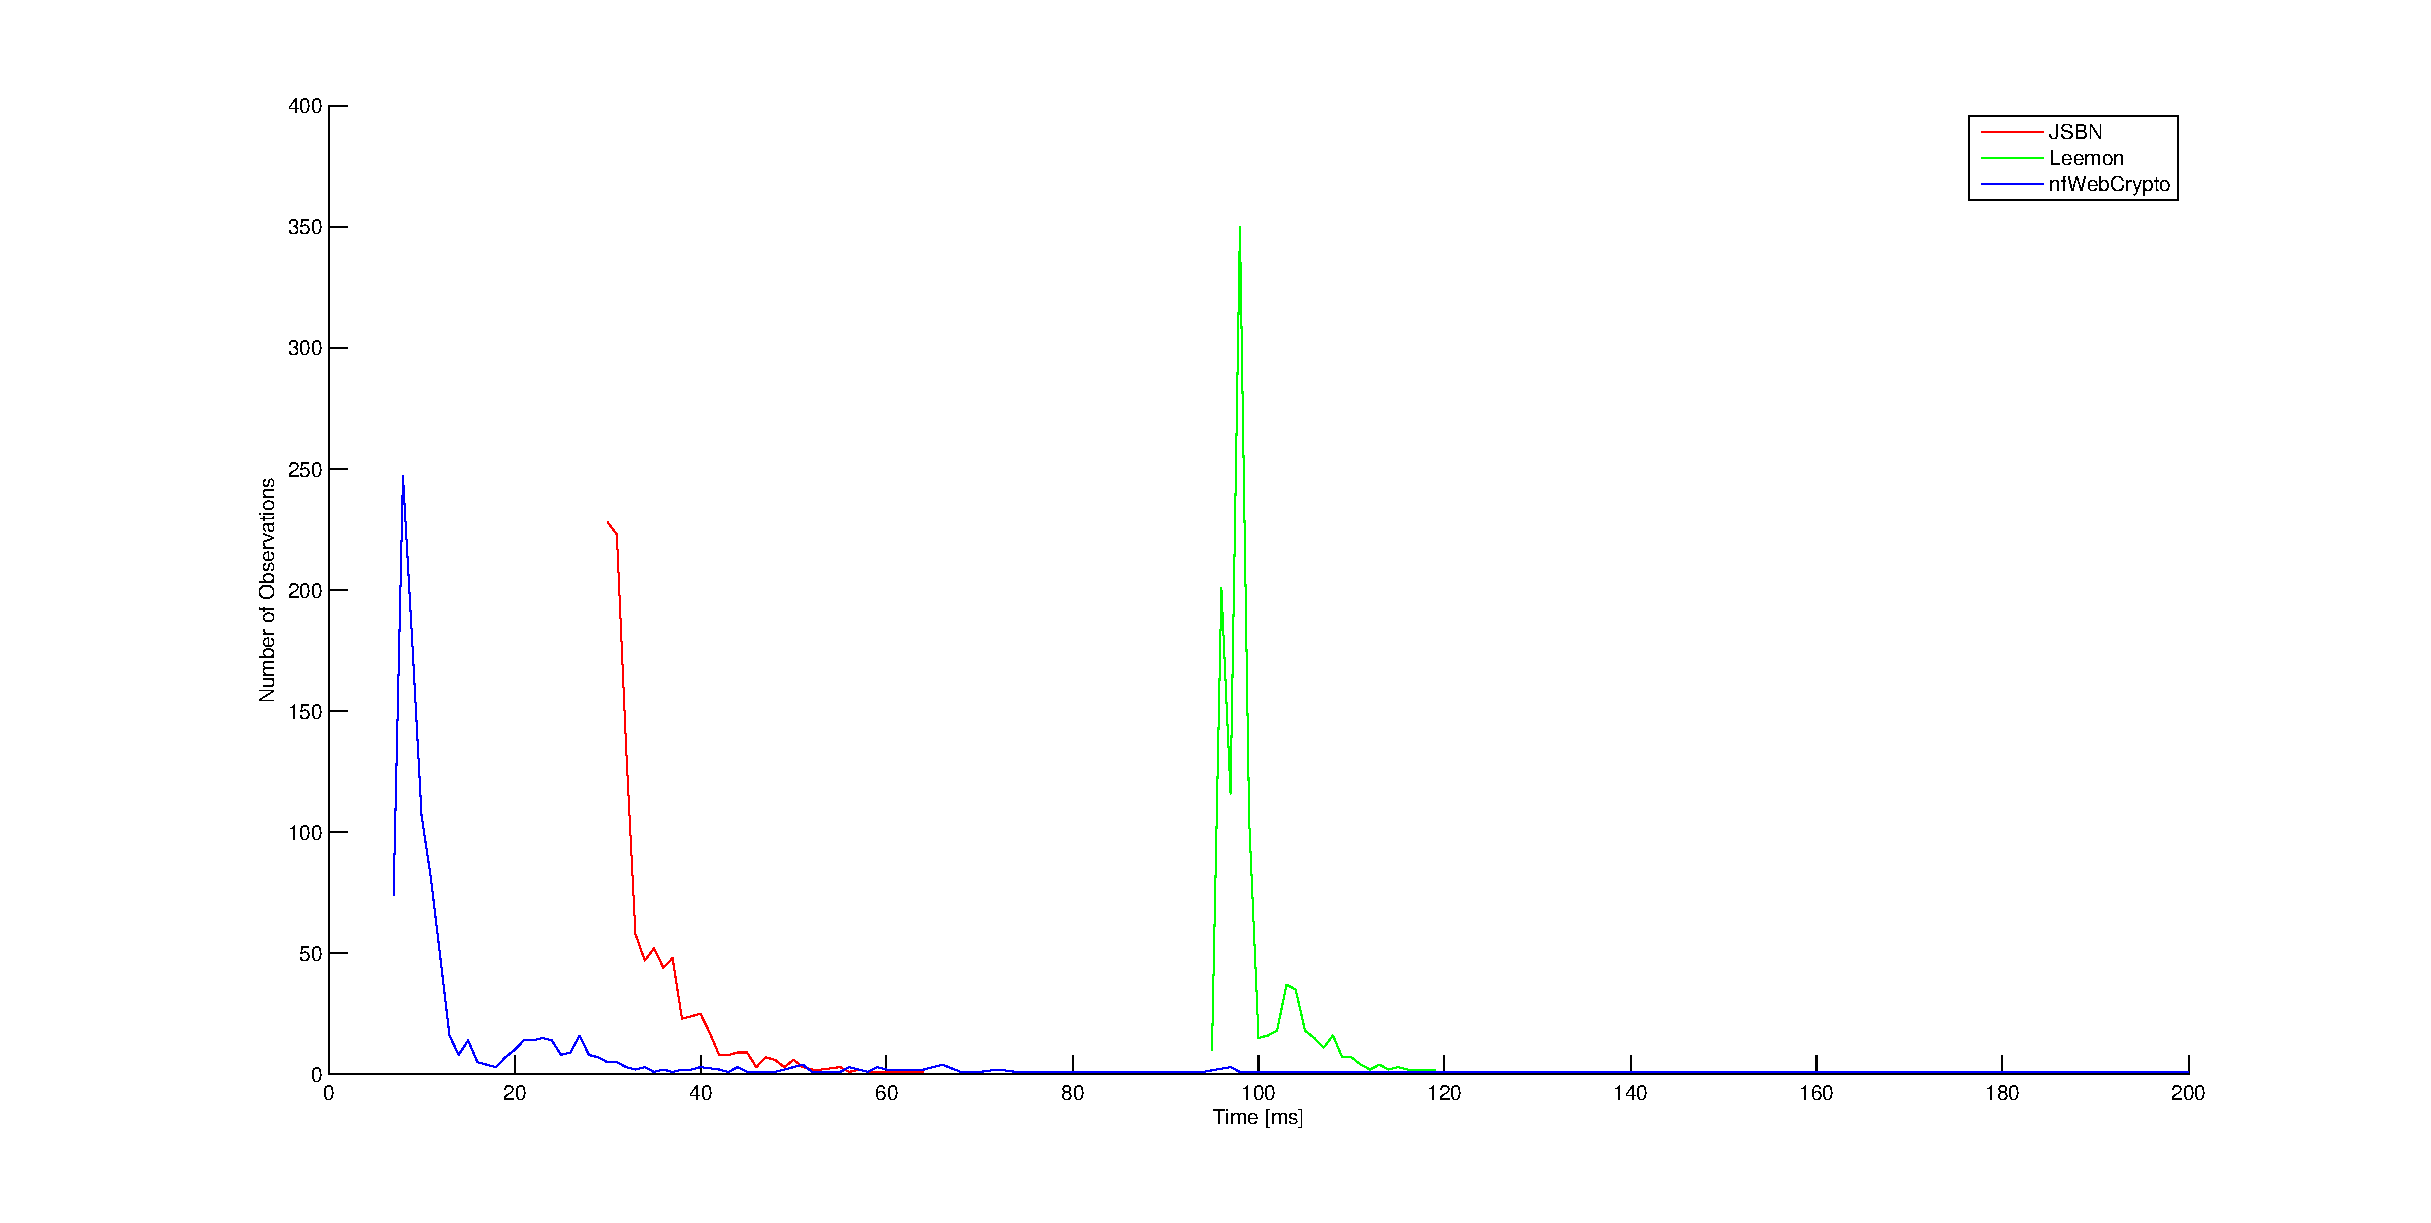
\includegraphics[width=\linewidth]{wc/modular_exponentiation.eps}}
  \caption{Modulaire exponentiatie}
  \label{fig:wc:modular_exponentiation}
\end{figure}

\begin{table}
  \begin{center}
    \begin{tabular}{r | c c}
      Library & Gemiddelde [ms] & Variantie [ms] \\ \hline
      JSBN & 33,9250 & 26,5019  \\
      Leemon & 99,1470 & 15,0785 \\
      NfWebCrypto & 16,0670 & 470,6251
    \end{tabular}
    \caption{Modulaire exponentiatie}
    \label{tab:wc:modular_exponentiation}
  \end{center}
\end{table}

\subsection{RSA}

\begin{figure}
  \center{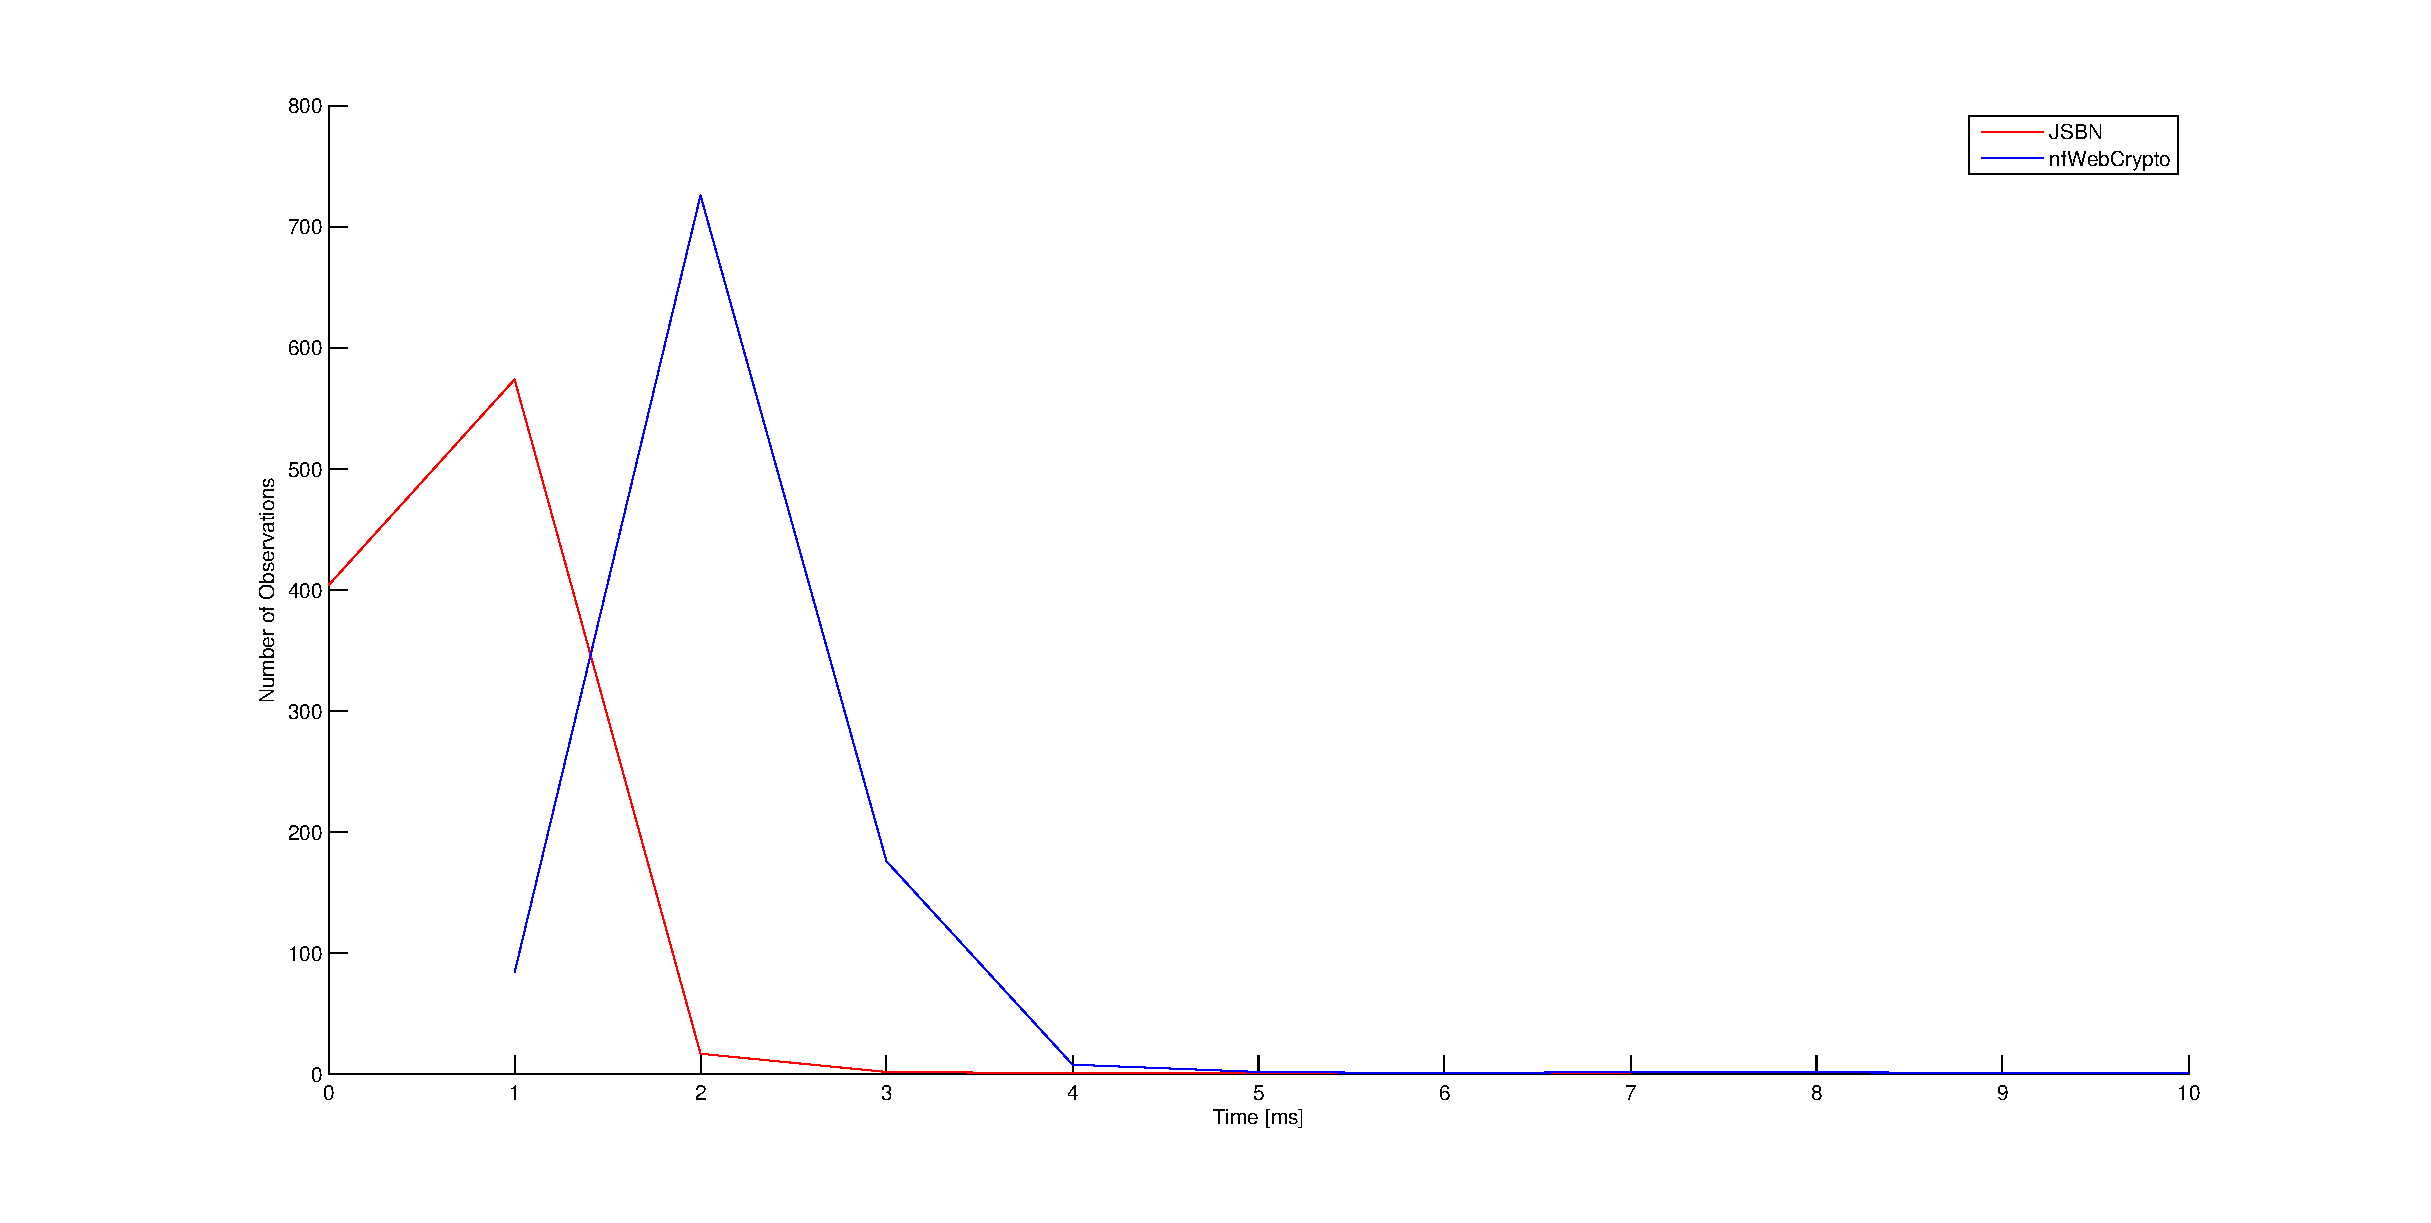
\includegraphics[width=\linewidth]{wc/rsa.eps}}
  \caption{RSA}
  \label{fig:wc:rsa}
\end{figure}

\begin{table}
  \begin{center}
    \begin{tabular}{r | c c}
      Library & Gemiddelde [ms] & Variantie [ms] \\ \hline
      JSBN & 0,6310 & 0,3632  \\
      NfWebCrypto & 2,1360 & 0,4219
    \end{tabular}
    \caption{RSA}
    \label{tab:wc:modular_exponentiation}
  \end{center}
\end{table}
